\apendice{Manual de Usuario}
\begin{center}
	
\includegraphics[scale=3]{logo.png}
\end{center}

\section{Tabla de contenido}\label{tabla-de-contenido}
\hyperref[objetivo-y-proceso]{Objetivo y proceso
\hyperref[objetivo-y-proceso]{2}}

\hyperref[administraciuxf3n]{Administración
	\hyperref[administraciuxf3n]{2}}

\hyperref[responsables]{Responsables \hyperref[responsables]{2}}

\hyperref[proyectos]{Proyectos \hyperref[proyectos]{3}}

\hyperref[convocatorias]{Convocatorias \hyperref[convocatorias]{4}}

\hyperref[solicitante]{Solicitante \hyperref[solicitante]{5}}

\hyperref[contratos]{Contratos \hyperref[contratos]{6}}

\hyperref[crear]{Crear \hyperref[crear]{6}}

\hyperref[renovaciuxf3n]{Renovación \hyperref[renovaciuxf3n]{7}}

\hyperref[renuncia]{Renuncia \hyperref[renuncia]{8}}

\hyperref[informes]{Informes \hyperref[informes]{10}}

\hyperref[nuxf3mina-mes]{Nómina-mes \hyperref[nuxf3mina-mes]{10}}

\hyperref[vencimientos]{Vencimientos \hyperref[vencimientos]{11}}

\hyperref[contratos-1]{Contratos \hyperref[contratos-1]{11}}

\hyperref[nominas-periodo]{Nominas-Periodo
	\hyperref[nominas-periodo]{12}}

\hyperref[acerca-de]{Acerca de \hyperref[acerca-de]{12}}

\hyperref[guuxeda-de-uso]{Guía de uso \hyperref[guuxeda-de-uso]{12}}

\section{Objetivo y proceso}\label{objetivo-y-proceso}

El objetivo de la aplicación \textbf{GeNomIn}, es la creación,
mantenimiento y gestión de las nóminas vinculadas a proyectos de
investigación generados por el Servicio de Investigación de la
Universidad de Burgos.

Para ello se ha establecido un proceso por el cual se irán desarrollando
los distintos elementos que conformar un contrato, desde el
mantenimiento de \textbf{Proyectos} e \textbf{Responsables}
(Investigadores), \textbf{Convocatorias}, \textbf{Solicitantes} de las
mismas, creación de \textbf{Contratos}, renovación y renuncia, y el
objetivo final que es la generación de \textbf{Informes} de nómina
mensuales, vencimientos de contratos y controles de nómina, para el
cotejo con los informes emitidos por el Servicio de Retribuciones que
actualmente se llevan con tablas Excel.

En esta guía de uso repasamos el proceso completo desde la
administración de proyectos y responsables hasta el informe final de
nómina mensual.

\section{Inicio de Sesión:}\label{inicio-de-sesiuxf3n}

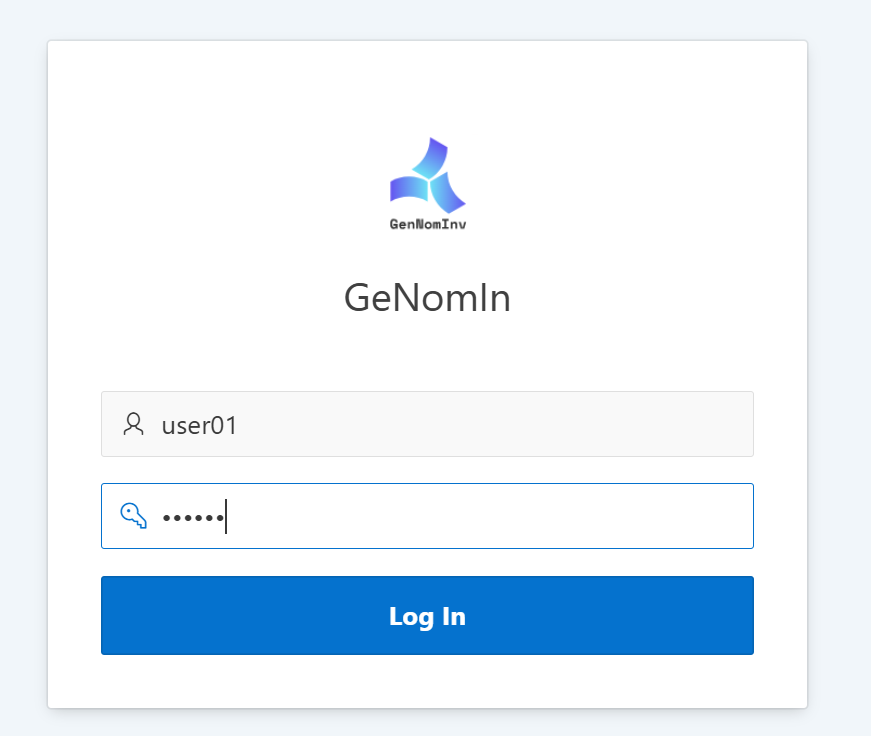
\includegraphics[width=2.39167in,height=2.02083in]{1.png}Una
vez accedida a la aplicación nos pedirá las credenciales de entrada, en
este caso accederemos con user01, user01.

Entrando al Menú principal, encontramos las siguientes opciones en el
Menú Lateral, \textbf{Aministración}, \textbf{Convocatorias},
\textbf{Contratos}, \textbf{Informes} y \textbf{Acerca de}, que pasamos a detallar.

También podremos volver al log inicial pulsando en el botón
\textbf{Salir}, de la derecha de la pantalla.

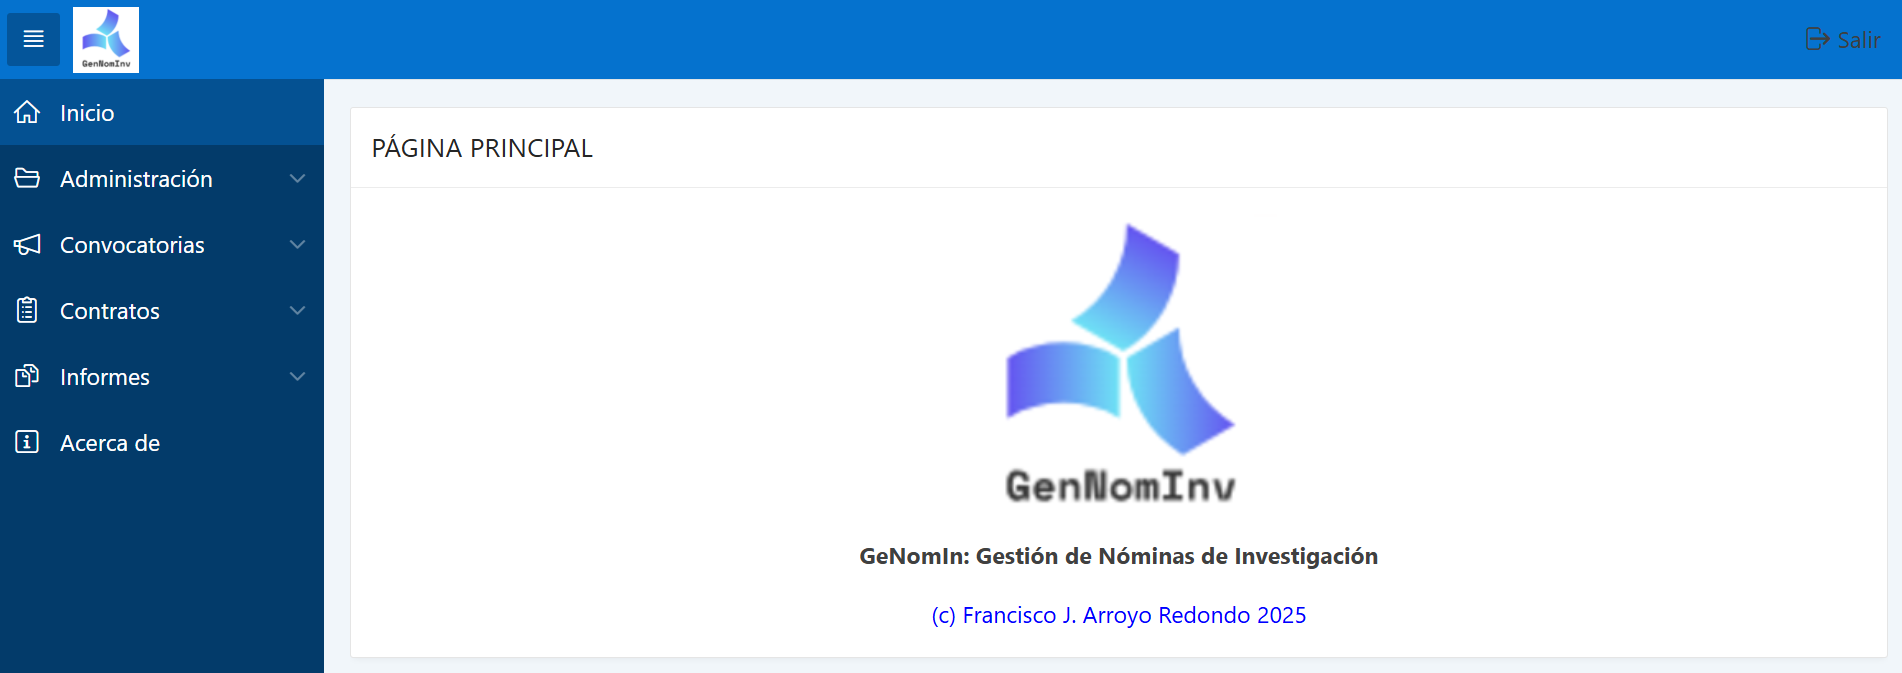
\includegraphics[width=5.90556in,height=2.08958in]{2.png}

\section{Administración}\label{administraciuxf3n}

Dentro del menú de \textbf{Administración}, podremos realizar la gestión
de los \textbf{Proyectos} y de los \textbf{Responsables} de los mismos

\subsection{Responsables}\label{responsables}

En esta tabla podemos ver y gestionar los Responsables de los proyectos,
indicar que todos estos datos, han sido generados aleatoriamente y no
corresponden a la realidad. Como vemos en la imagen,
podremos Buscar por campos, (pulsando en el icono de la lupa ) , editar los datos (pulsando en el icono del lápiz ), crear, agrupaciones, filtros, informes y descargarlos, pulsando en el botón \textbf{Actions}.

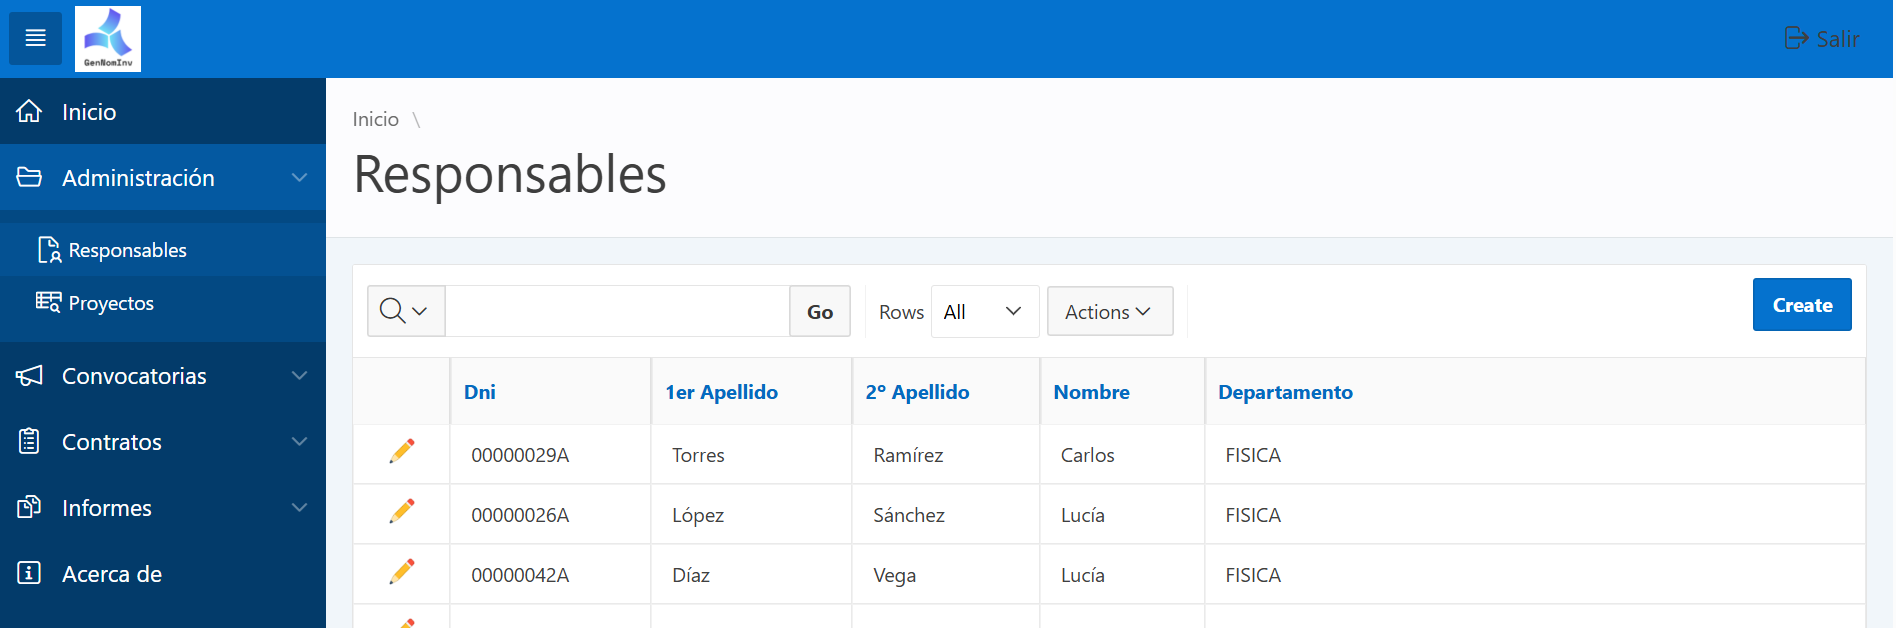
\includegraphics[width=5.90556in,height=1.95625in]{3.png}

Si lo que queremos es crear un nuevo responsable pulsaremos en la opción
\textbf{Create} de la derecha, que nos mostrará el siguiente menú, donde
podremos incluir los datos necesarios, DNI, Apellidos, Nombre y
Departamento (el cual podremos escoger en la cortinilla desplegable)

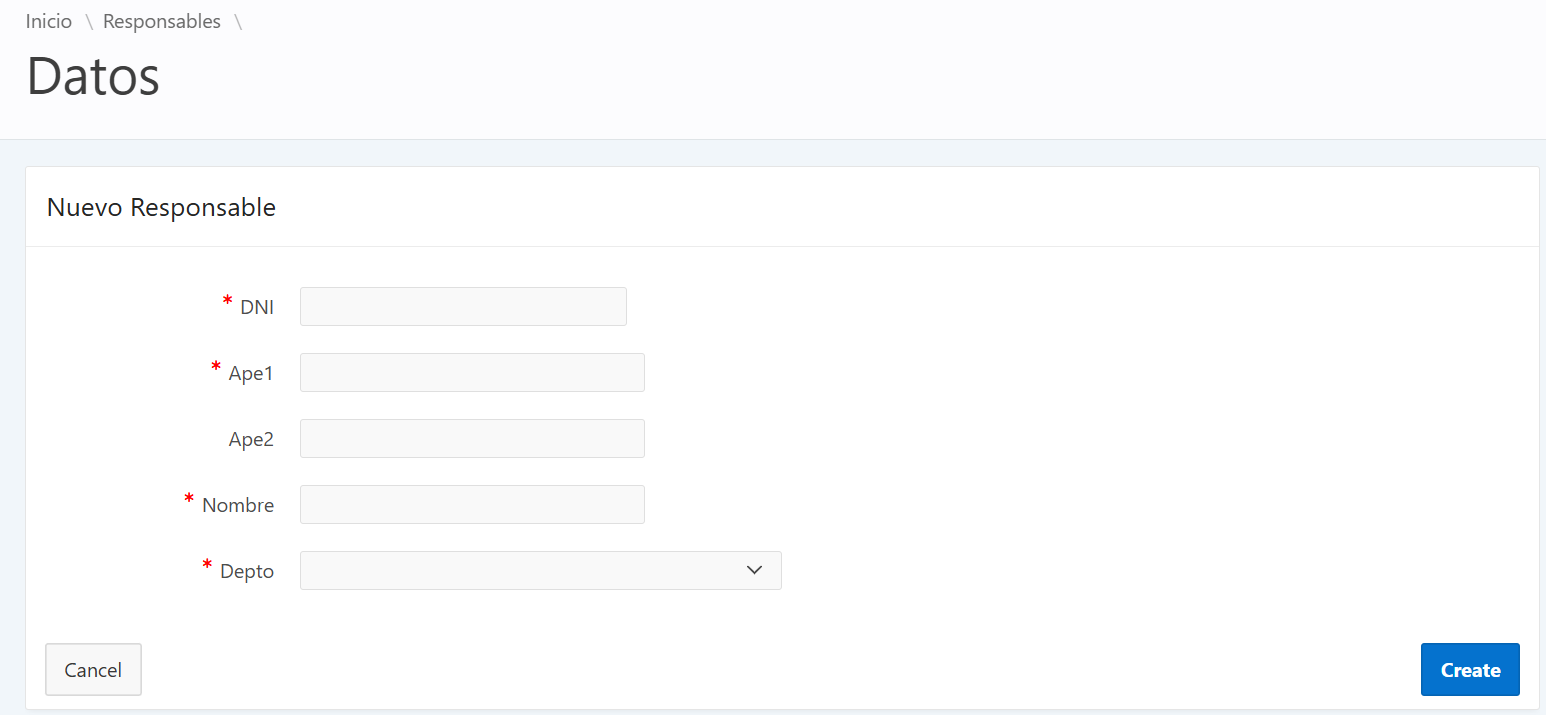
\includegraphics[width=5.90556in,height=2.73125in]{4.png}

\subsection{Proyectos}\label{proyectos}

Para los proyectos se ha creado un Grid Interactivo, que muestra los
proyectos existentes (éstos también han sido generados de forma
aleatoria), realizar búsquedas por Orgánica, Titulo y Resposable, editar
campos, añadir nuevos proyectos (\textbf{Add Row}) y desde el botón
\textbf{Actions}, generar filtros e informes.

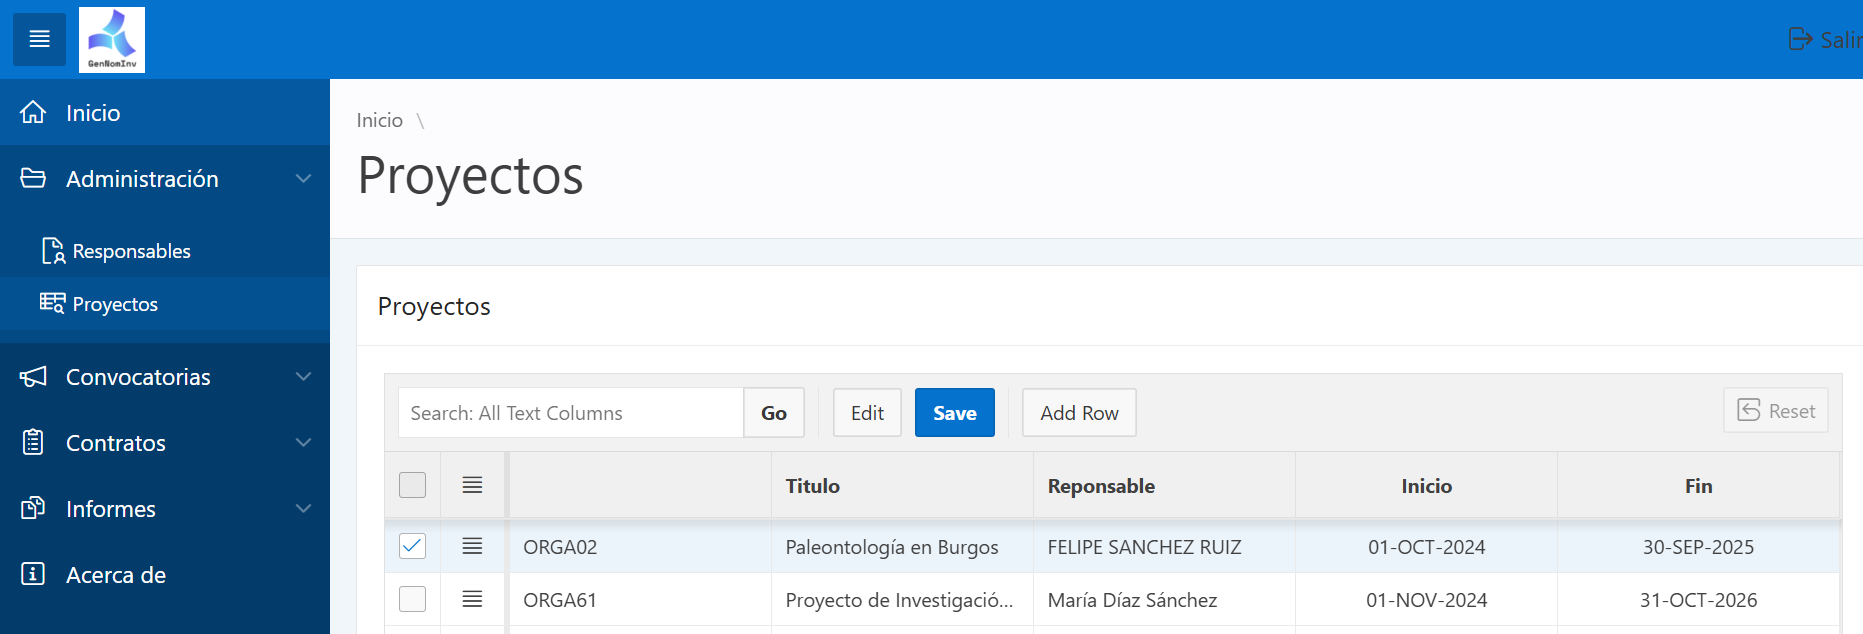
\includegraphics[width=5.90556in,height=1.97083in]{5.png}

\section{Convocatorias}\label{convocatorias}

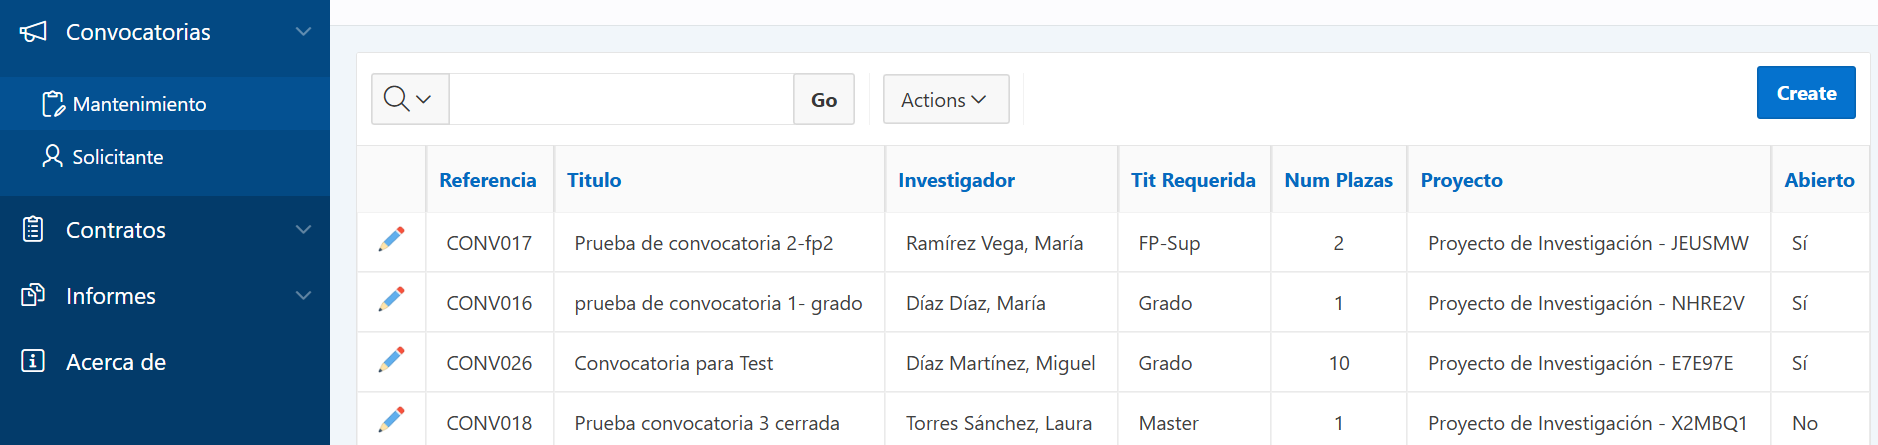
\includegraphics[scale=1]{6.png}
Desde el menú convocatorias, podremos realizar el \textbf{Mantenimiento} de las convocatorias que solicite un Responsable de un Proyecto, inicialmente nos mostrará todas las que tenemos pudiendo editarlas, pulsando el icono del lapicero

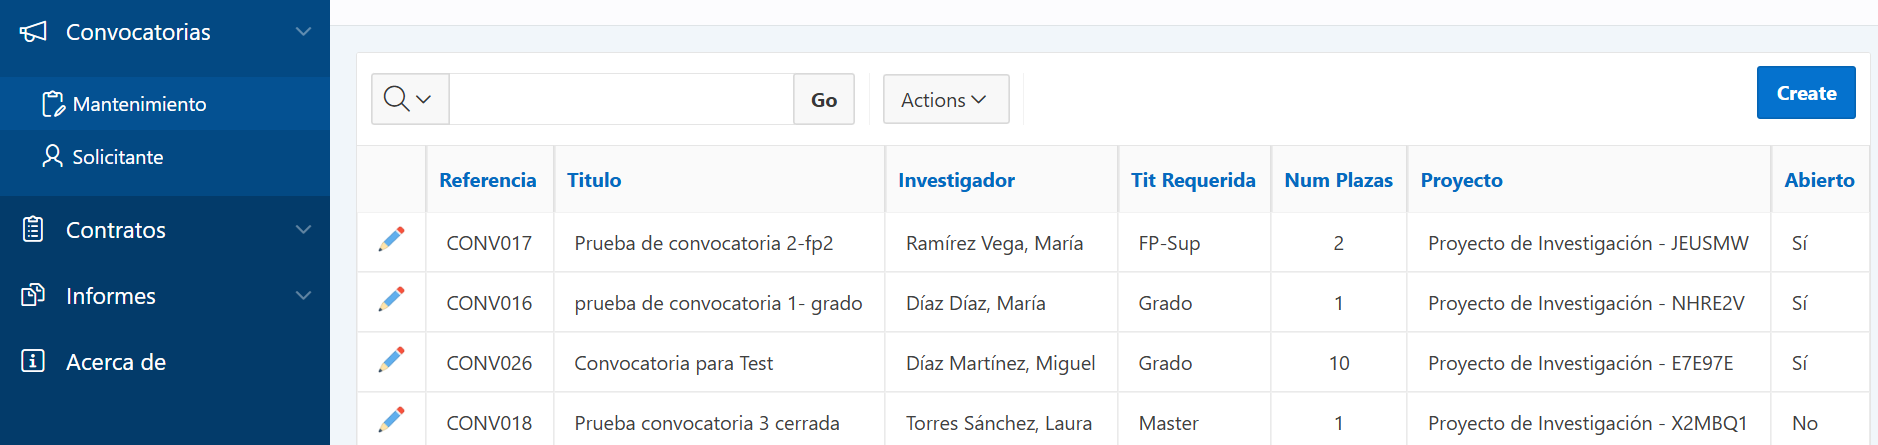
\includegraphics[scale=1]{7.png}
También podremos hacer búsquedas por los distintos campos, pulsando como en anteriores ocasiones en la lupa y las mismas acciones.

Para generar una nueva convocatoria pulsaremos en el botón
\textbf{Create}:

Tendremos que rellenar los campos que se indican obligatoriamente con un *

En el desplegable \textbf{Tit Requerida}, podremos seleccionar una de las titulaciones mínima que se requerirán para poder optar, por los solicitantes a cada convocatoria.

En el desplegable \textbf{Investigador}, podremos seleccionar cualquiera de los investigadores que estén dados de alta en el sistema, como hemos visto anteriormente en la pantalla \textbf{Responsables}. Este punto es importante, ya que en siguiente desplegable \textbf{Ref. Proy}, solo nos mostrará los proyectos del investigador seleccionado, indicándonos después el tiempo que queda para la finalización de este proyecto.

Al confirmar con \textbf{OK} podremos pulsar en el botón
\textbf{Create}, generando una nueva convocatoria.

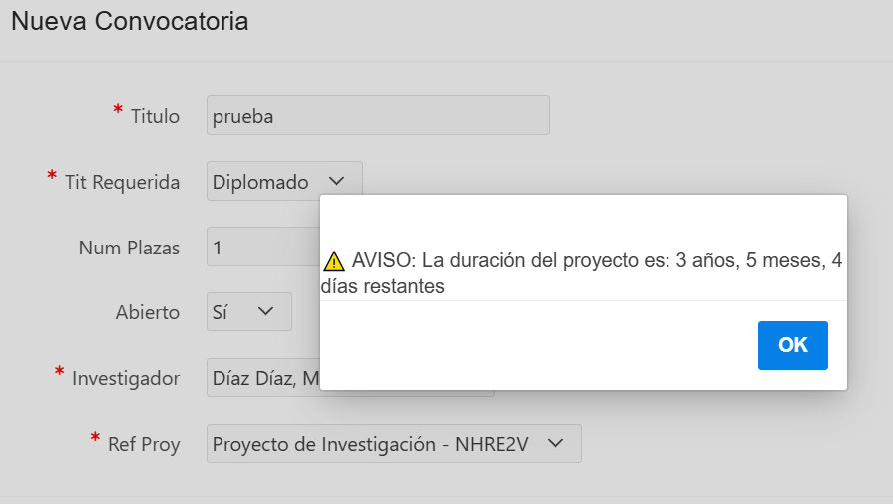
\includegraphics[scale=1]{8.png}

\subsection{Solicitante}\label{solicitante}

Esta pantalla nos mostrará los solicitantes existentes para las
convocatorias creadas, pudiendo realizar las mismas operaciones que
anteriormente (búsquedas por campos y diversas acciones)

También podremos dar de alta un nuevo solicitante de una convocatoria
abierta, pulsando en el botón \textbf{Create}.

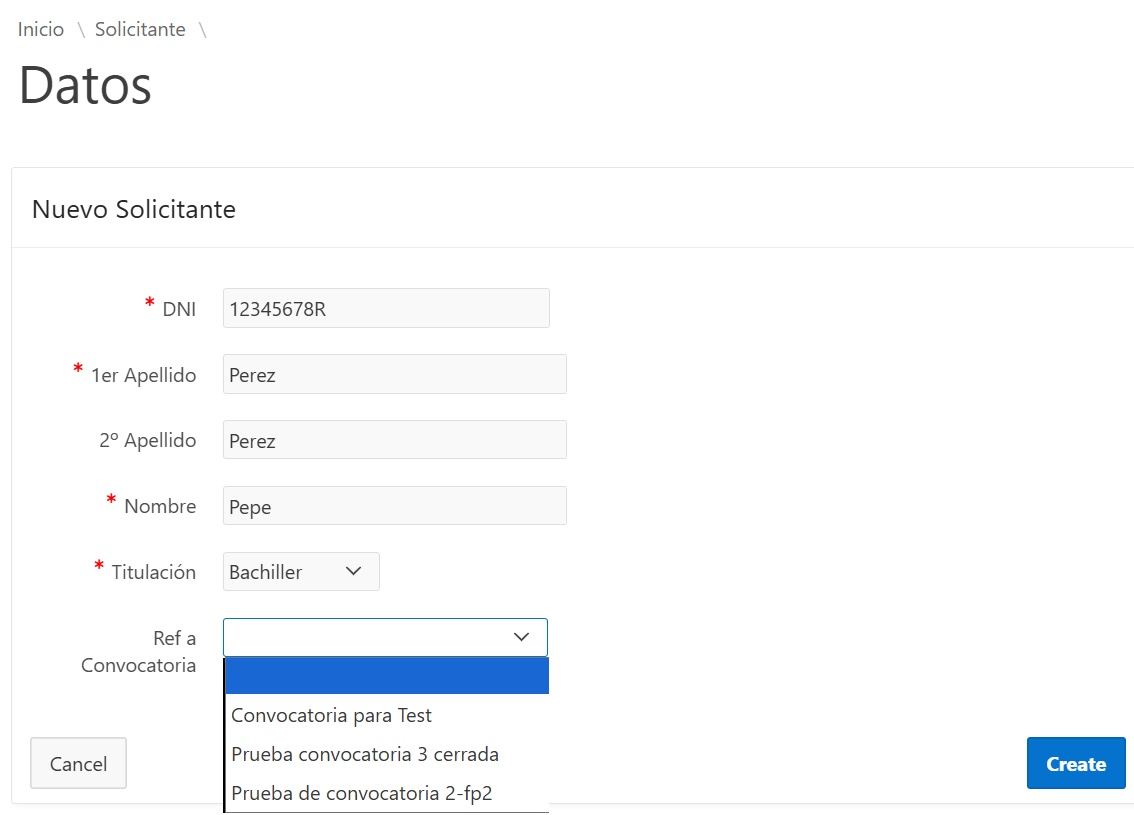
\includegraphics[scale=1]{9.png}


Tendremos que rellenar los campos que se indican y seleccionar en el desplegable \textbf{Titulación}, una de las opciones que se indican correspondiente al nivel académico del solicitante.
Luego escogeremos la convocatoria en la que quiere participar, y al
seleccionarla, el sistema nos informará si puede o no participar, según el nivel requerido para la misma. En este caso con un nivel de Bachiller, en la convocatoria para Test, nos avisa de la incidencia.

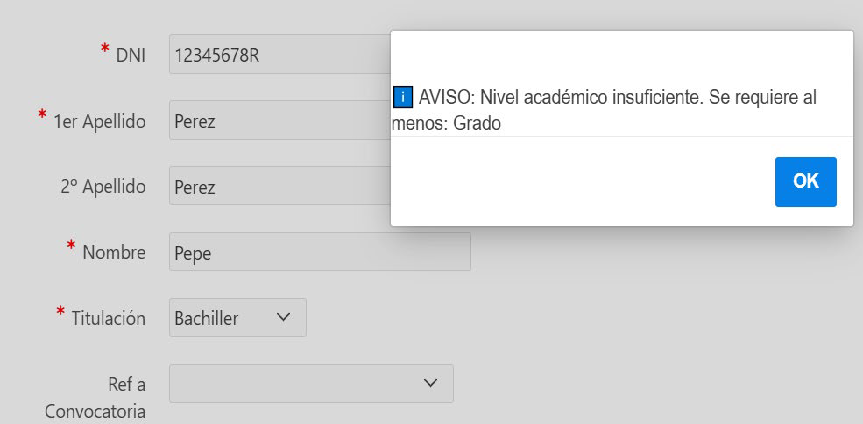
\includegraphics[scale=1]{10.png}

También, nos indicará si la convocatoria ya está cerrada, es el caso de si escogemos la opción de convocatoria cerrada.

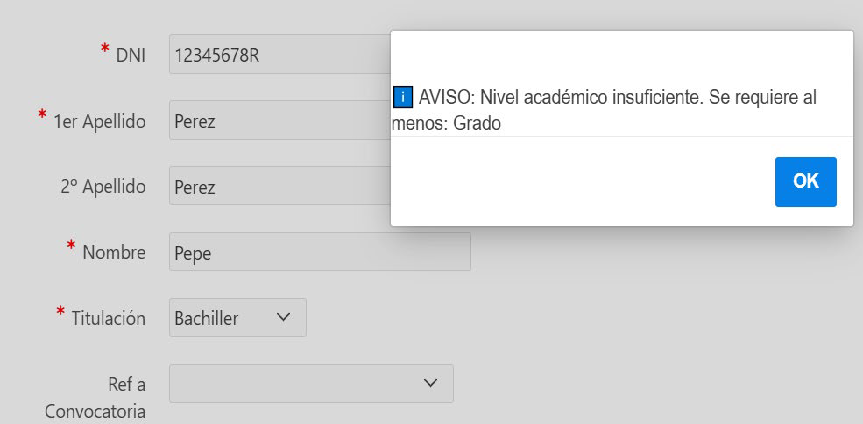
\includegraphics[scale=1]{11.png}

Si la convocatoria fuera adecuada a su titulación pulsaríamos el botón \textbf{Create}

\section{Contratos}\label{contratos}

\subsection{Crear}\label{crear}

Dentro de esta opción podremos \textbf{Crear}, un contrato para un
\textbf{Solicitante}, vinculado a una \textbf{Convocatoria}

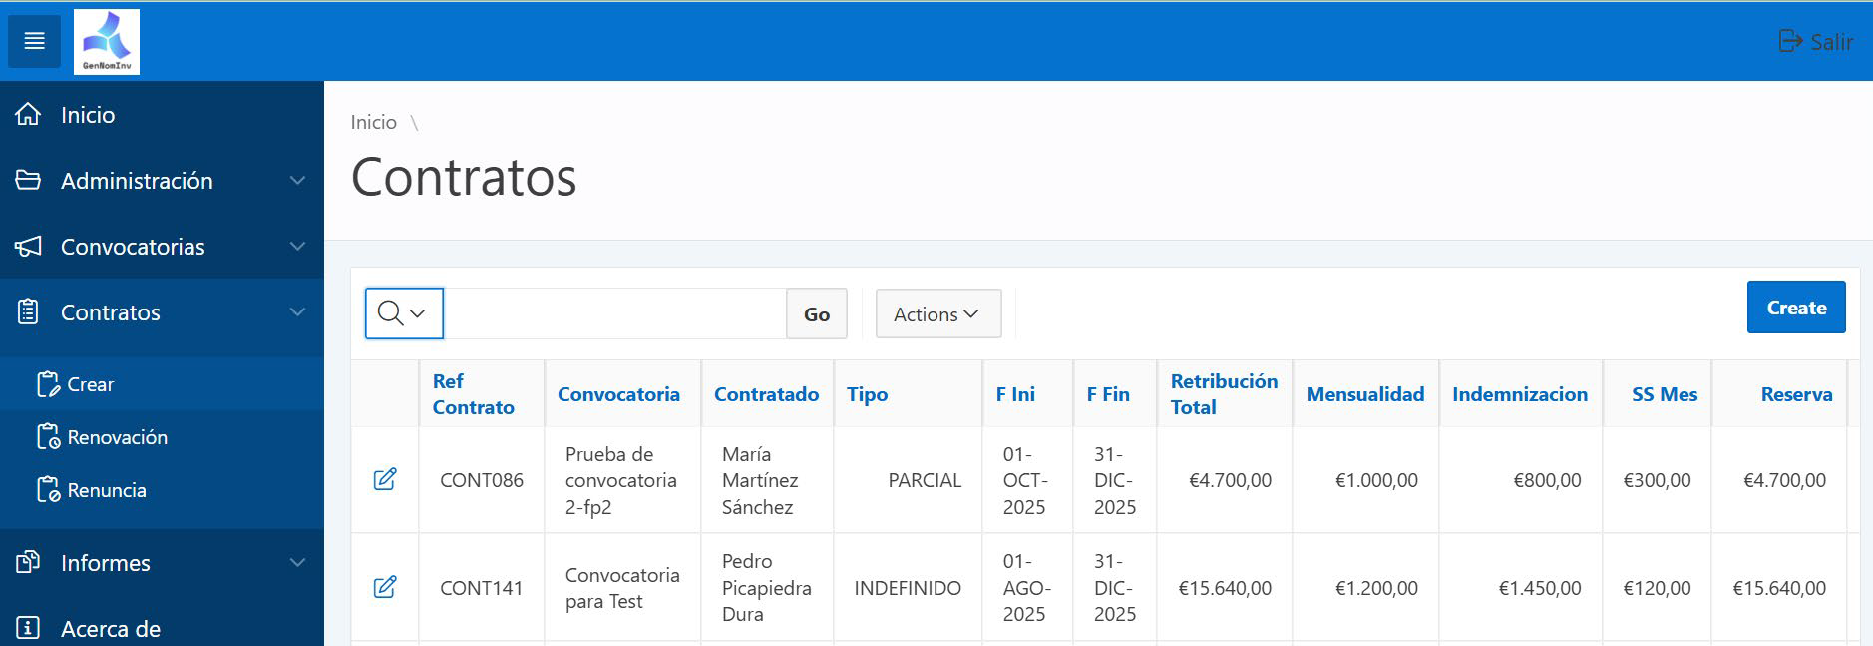
\includegraphics[scale=1]{13.png}

Inicialmente vemos los contratos dados de alta, pudiendo realizar las distintas tareas como en anteriores ocasiones, tales como, búsquedas por campos y diversos filtros e informes. Además, pulsando en el icono de edición podremos modificar datos de un contrato.

Para generar un nuevo contrato, pulsaremos en el botón \textbf{Create}

Inicialmente nos solicitará para qué convocatoria queremos el contrato, mostrando aquellos solicitantes de esa convocatoria.

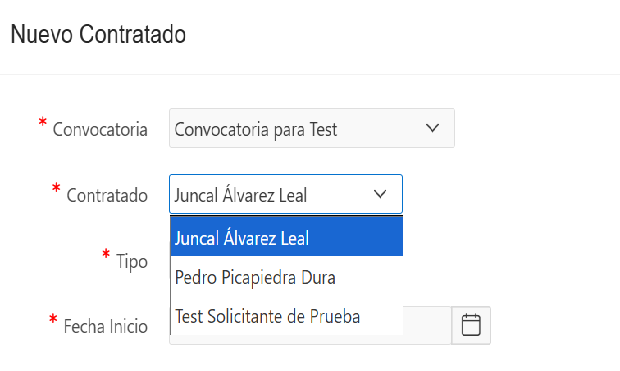
\includegraphics[scale=1]{14.png}

Luego nos irá solicitando los diversos datos para realizar el contrato.

En el desplegable \textbf{Tipo}, podremos escoger entre los distintos tipos de contrato en vigor.

Después deberemos introducir las fechas de inicio y fin, las cuales
deberán estar comprendidas entre las fechas del \textbf{Proyecto}
vinculado, lanzando sendos avisos si no se cumpliera este requisito:

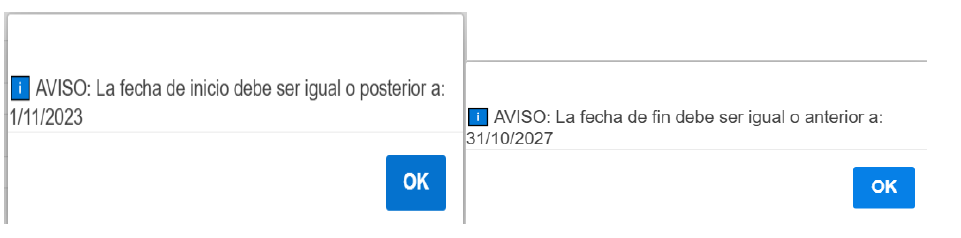
\includegraphics[scale=1]{15.png}

Una vez introducidos los datos requeridos y pulsando en el botón
\textbf{Create}, nos pedirá confirmación para la creación del nuevo
contrato y de la generación las nóminas correspondientes en la tabla nómina automáticamente para los meses correspondientes y uno adicional de seguridad social, que no tiene retribución.

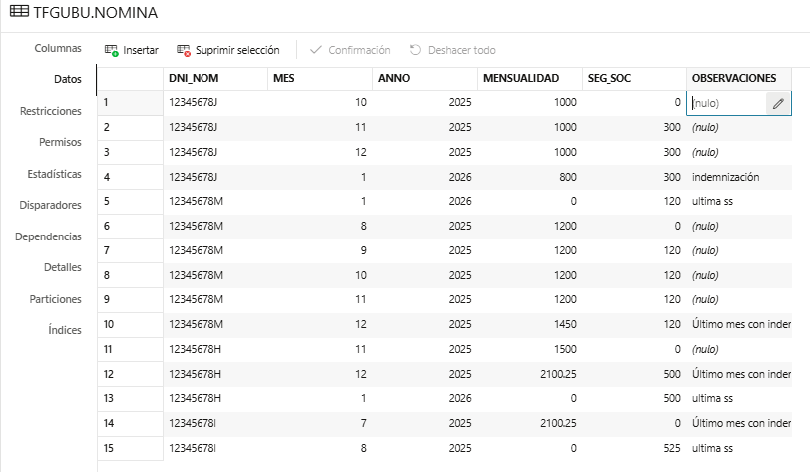
\includegraphics[width=5.90556in,height=3.43958in]{16.png}

\subsection{Renovación}\label{renovaciuxf3n}

En este apartado podremos realizar la renovación de un contrato, siempre y cuando no sobrepase la fecha fin del \textbf{Proyecto}, vinculado.

Así, al seleccionar un contrato, nos ofrecerá los datos del mismo en la parte izquierda:

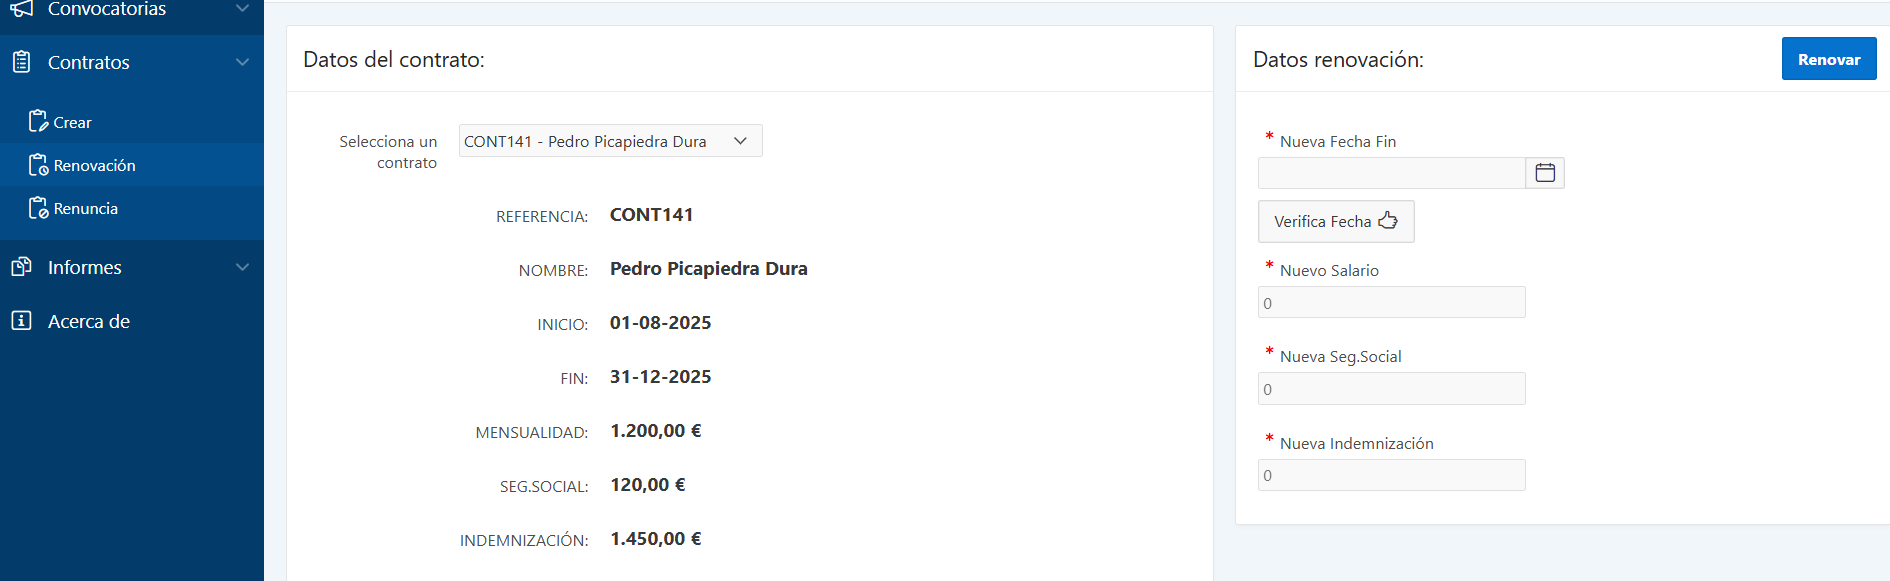
\includegraphics[width=5.90556in,height=1.81528in]{17.png}

Pudiendo introducir los datos en la parte derecha.

Para la fecha de renovación deberemos verificar la misma, pulsando en el botón \textbf{Verifica Fecha}, indicándonos si por ejemplo la fecha es anterior a la actual:

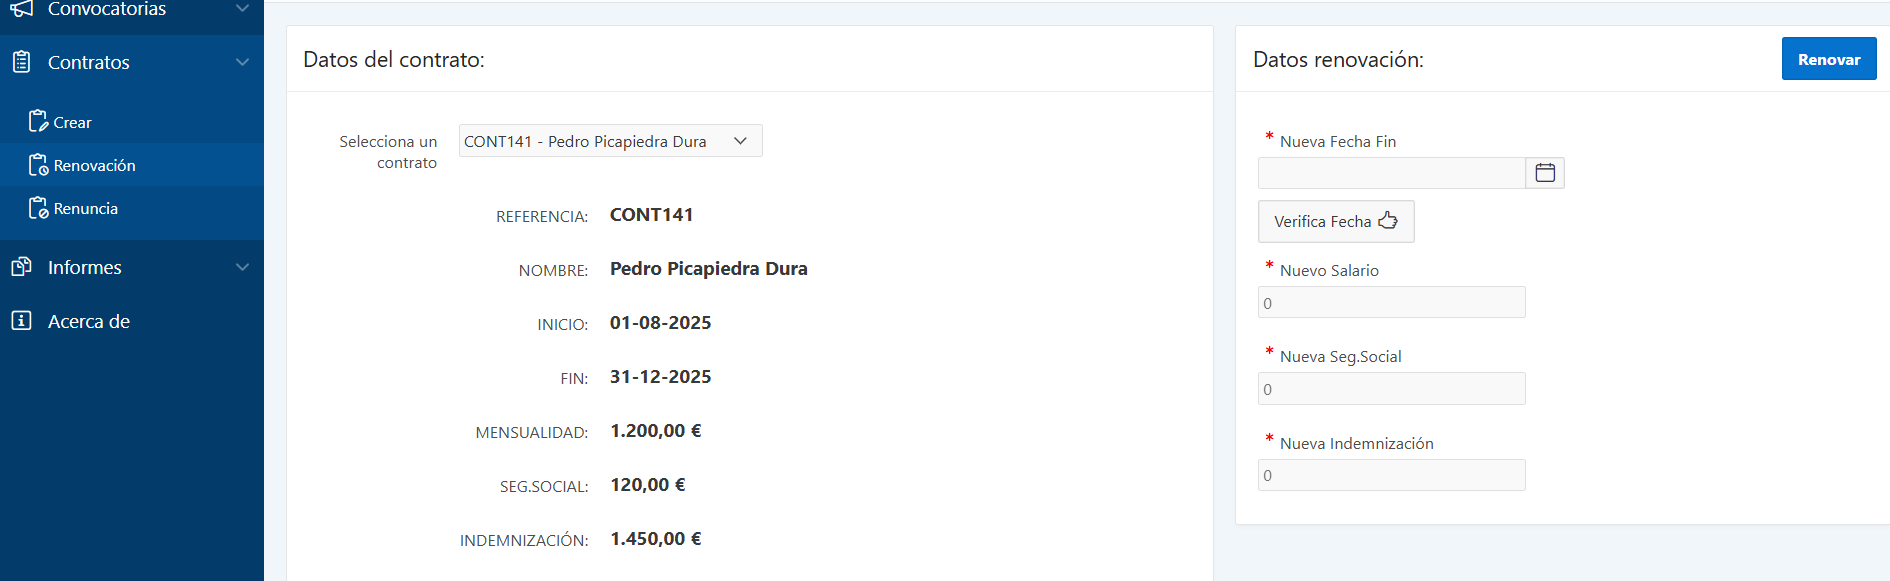
\includegraphics[width=2.59028in,height=0.98611in]{18.png}

Si la fecha excede del fin del contrato o si la fecha fuese correcta, el botón cambiará a color verde.

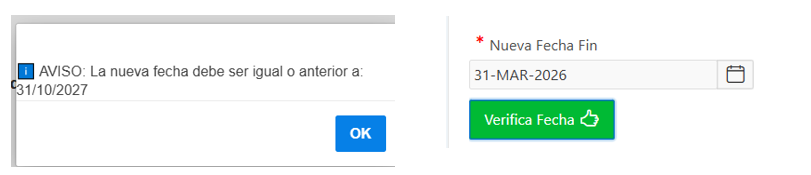
\includegraphics[scale=1]{19.png}

Una vez rellenos los datos correspondientes y pulsado el botón
\textbf{Renovar}, nos solicitará confirmación, como en el caso de
creación inicial y generará las nuevas nóminas correspondientes y
cambiará la fecha fin del mismo.

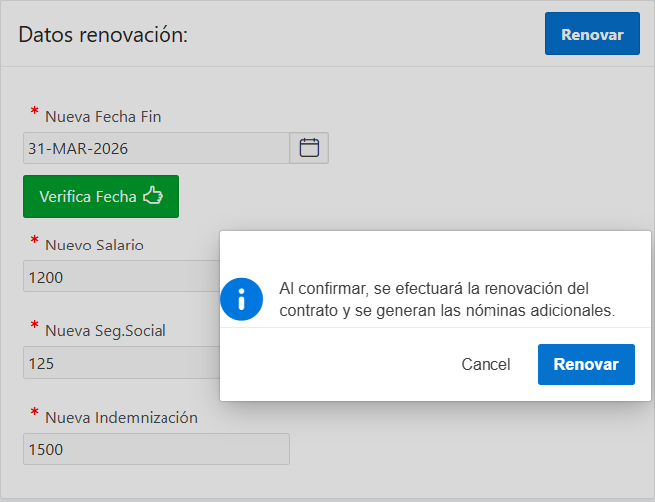
\includegraphics[width=4.25526in,height=3.25799in]{20.png}

Realizando la confirmación:


\includegraphics[width=5.90556in,height=0.99653in]{21.png}

\subsection{Renuncia}\label{renuncia}

En esta sección un solicitante podrá renunciar a un contrato en una
fecha determinada.

Como en el caso de la \textbf{Renovación}, tendremos que  seleccionar un contrato:

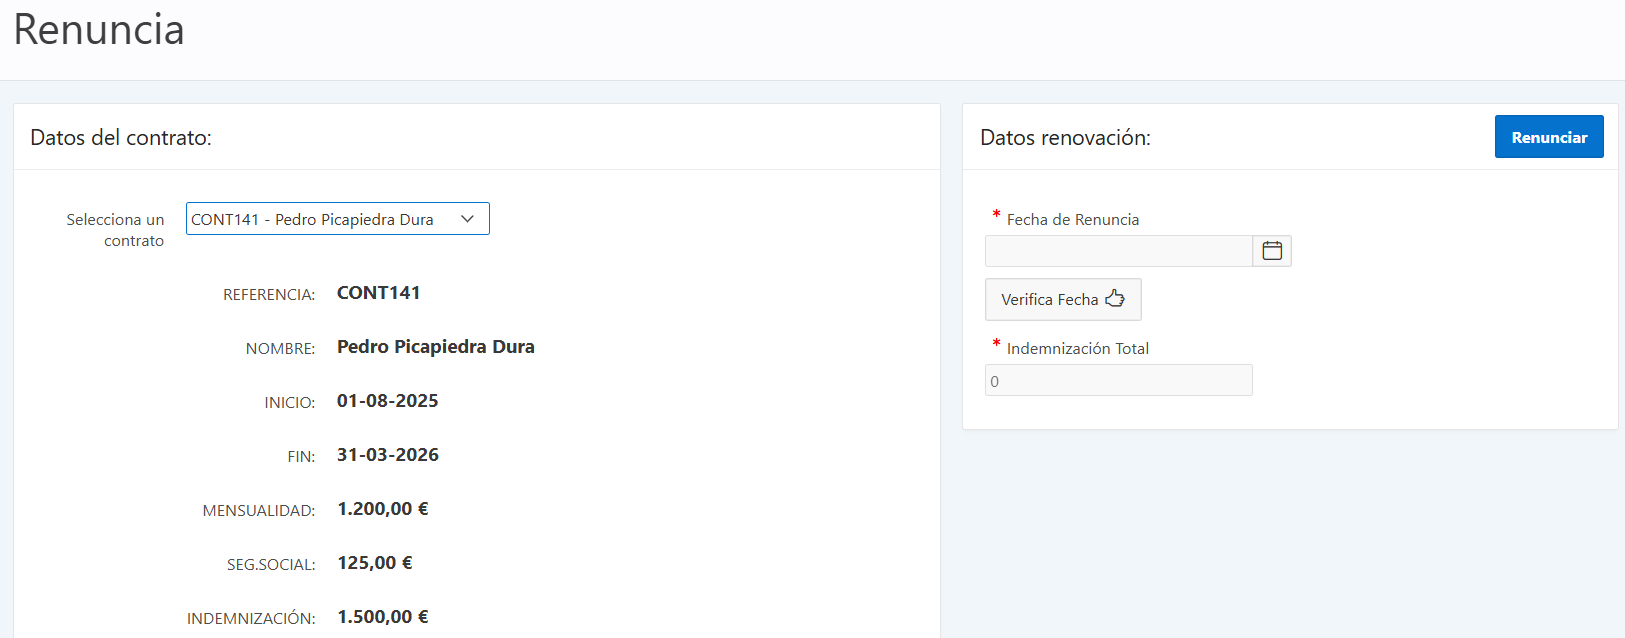
\includegraphics[width=5.90556in,height=2.31875in]{22.png}

El sistema nos mostrará los datos del contrato y la fecha fin actual, debiendo introducir en la parte de la derecha los datos de renuncia, y como en el caso anterior, comprobando si la renuncia es posterior a la fecha actual.

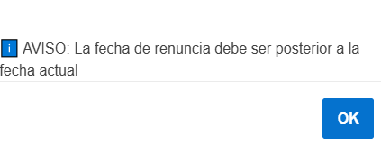
\includegraphics[width=2.32222in,height=0.90208in]{23.png}

Y si es anterior a la fecha fin actual.


\includegraphics[width=2.47222in,height=0.93681in]{24.png}

En el caso de haber introducido una fecha de renovación correcta, se verifica, con el botón en verde y al completar el resto de datos
podremos pulsar en el botón \textbf{Renunciar}

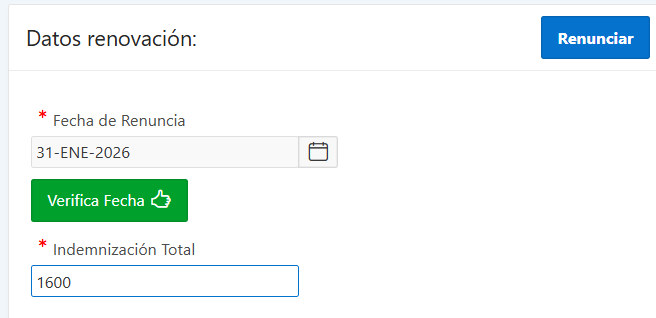
\includegraphics[width=5.90556in,height=2.8625in]{25.png}

En este momento se nos pedirá confirmación para realizar la acción, que eliminará las nóminas correspondientes y cambiará la fecha fin del contrato.

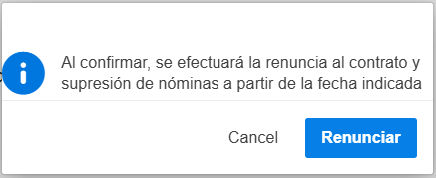
\includegraphics[width=3.73277in,height=1.52044in]{26.png}

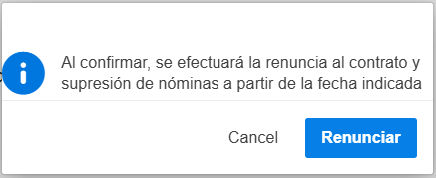
\includegraphics[width=5.90556in,height=0.89028in]{27.png}

\section{Informes}\label{informes}

\subsection{Nómina-mes}\label{nuxf3mina-mes}

Con este informe podremos ver la nómina correspondiente al mes seleccionado, es el informe principal de la aplicación, ya que se compara con la sábana de retribuciones y se coteja con los datos obrantes en el servicio. Para ello accedemos a la sección de informes Nómina-mes y muestra la pantalla siguiente, en la que podemos escoger mes y año y al pulsar en Consultar obtendremos las nóminas a pagar ese mes.

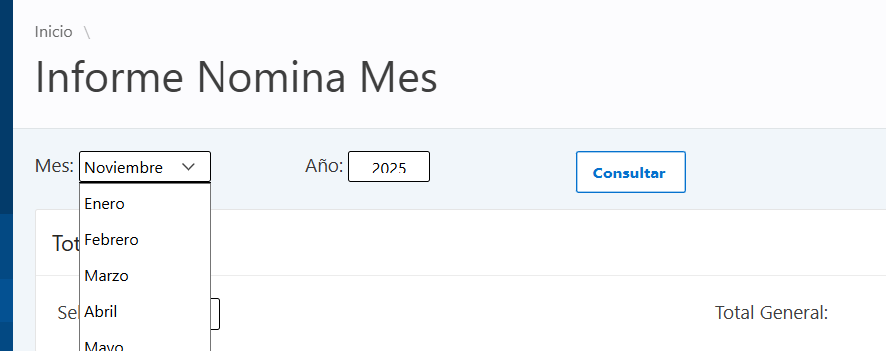
\includegraphics[width=4.11806in,height=1.6324in]{28.png}

Una vez mostrados los datos, podremos filtrar por orgánica y volver a pulsar Consultar para aplicar ese filtro.

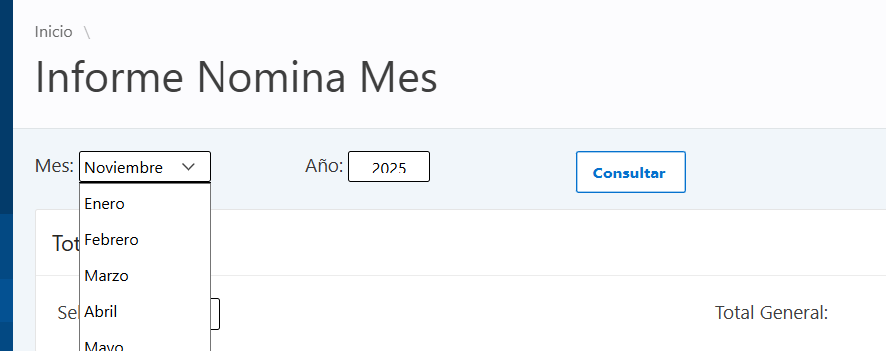
\includegraphics[width=5.15117in,height=2.55014in]{29.png}

Una vez conforme la vista pulsando en el botón generar, nos descargará un informe personalizado en pdf a través del servicio online Appex Oficce Print (AOP).

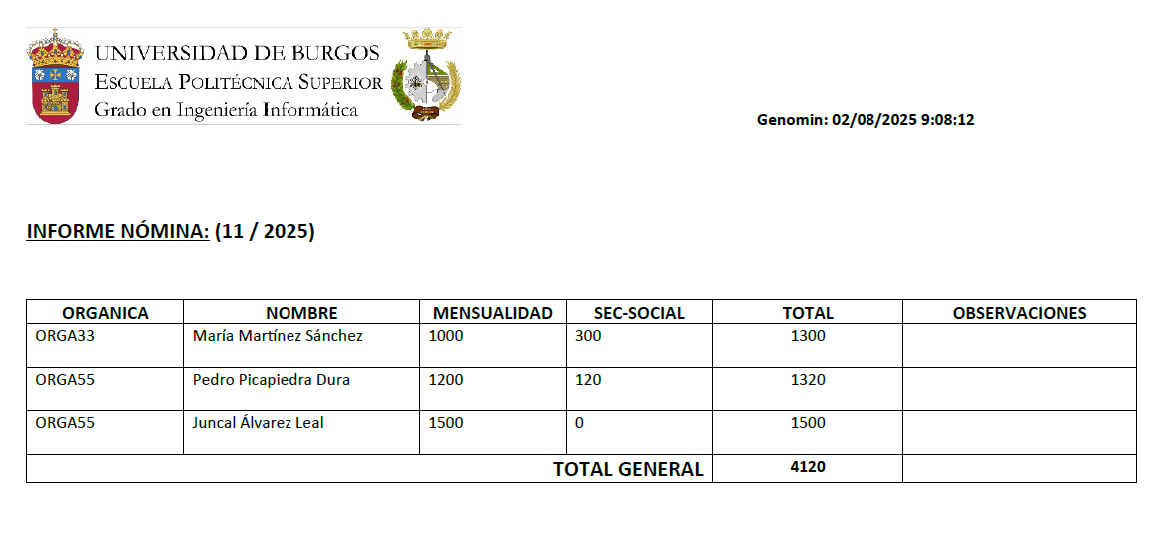
\includegraphics[width=5.90556in,height=2.73889in]{30.png}

\subsection{Vencimientos}\label{vencimientos}

Desde aquí podremos consultar los vencimientos de los contratos, para ello introduciremos la fecha inicio y fin y pulsaremos el botón Consulta:

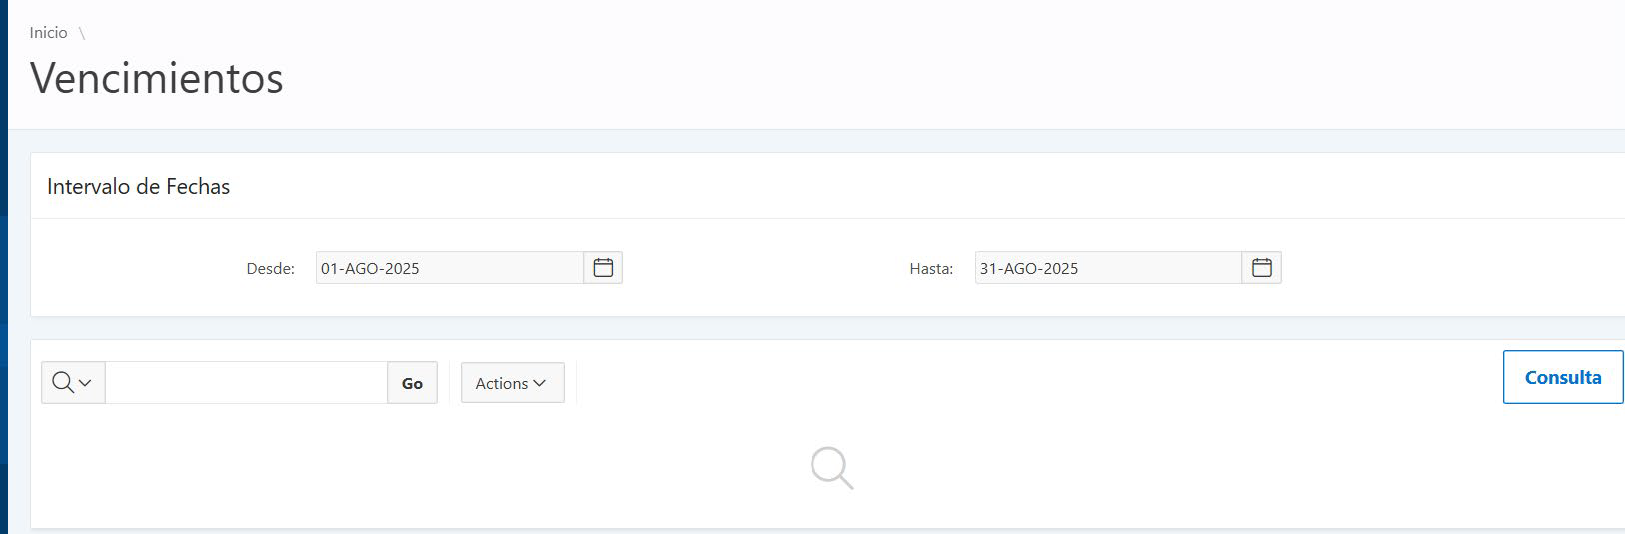
\includegraphics[width=5.90556in,height=1.93958in]{31.png}

Que nos mostrará los contratos que vencen entre las fechas indicadas:

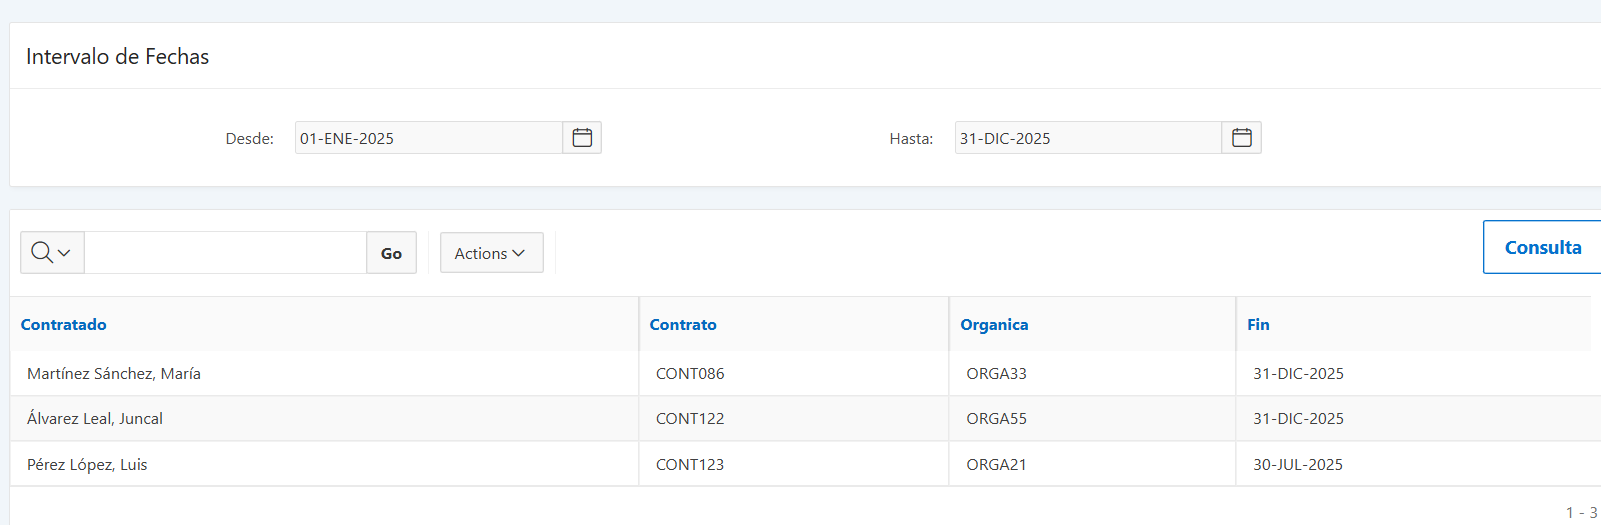
\includegraphics[width=5.90556in,height=1.93681in]{32.png}

Pulsando en la lupa podremos filtrar por campos y en el botón Actions, nos permite realizar varias opciones; como columnas a mostrar, filtros avanzados, ordenar datos y operar, guardar este informe para otras ocasiones (si lo hemos modificado) y descargar el informe en varios formatos

\subsection{Contratos}\label{contratos-1}

Este informe ofrece un listado de todos los datos de los contratos que hay en vigor

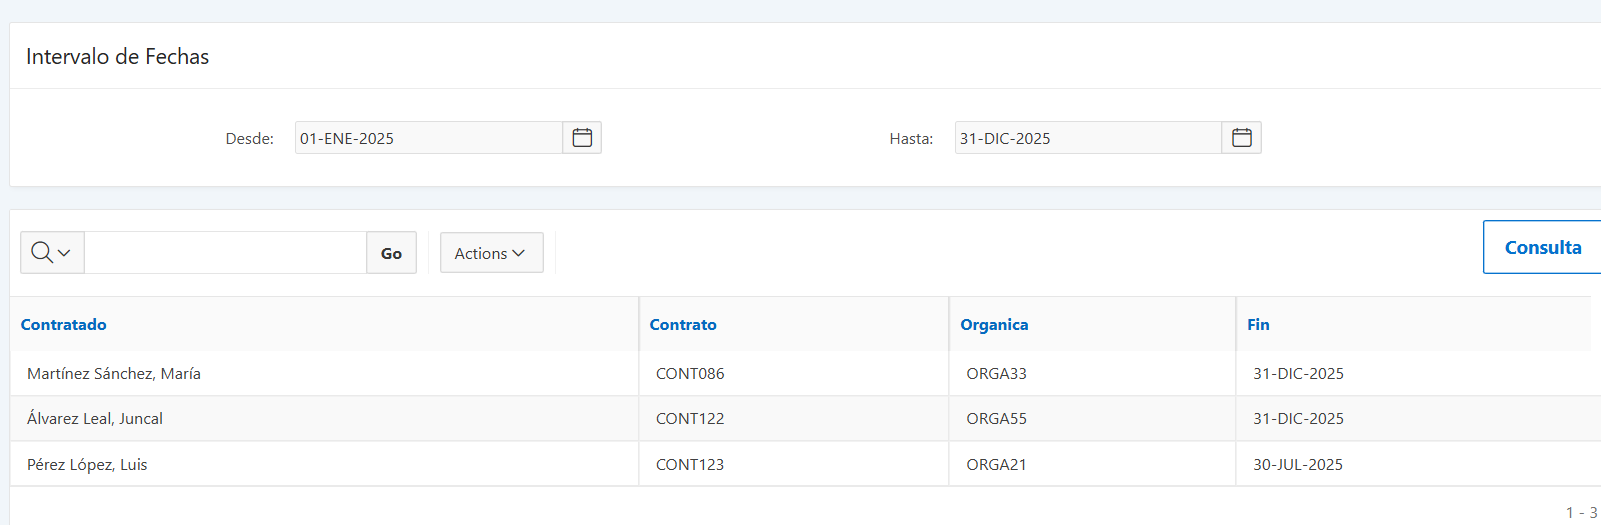
\includegraphics[width=5.90556in,height=1.58889in]{33.png}

Como en el anterior informe se pueden filtrar campos con la lupa y
acceder a otras opciones y filtros avanzados con el botón Actions.

\subsection{Nominas-Periodo}\label{nominas-periodo}

Este informe presenta las nóminas que tiene un contratado en un periodo que se indica, una vez accedido al informe tendremos que seleccionar el contratado y el periodo desde, hasta.

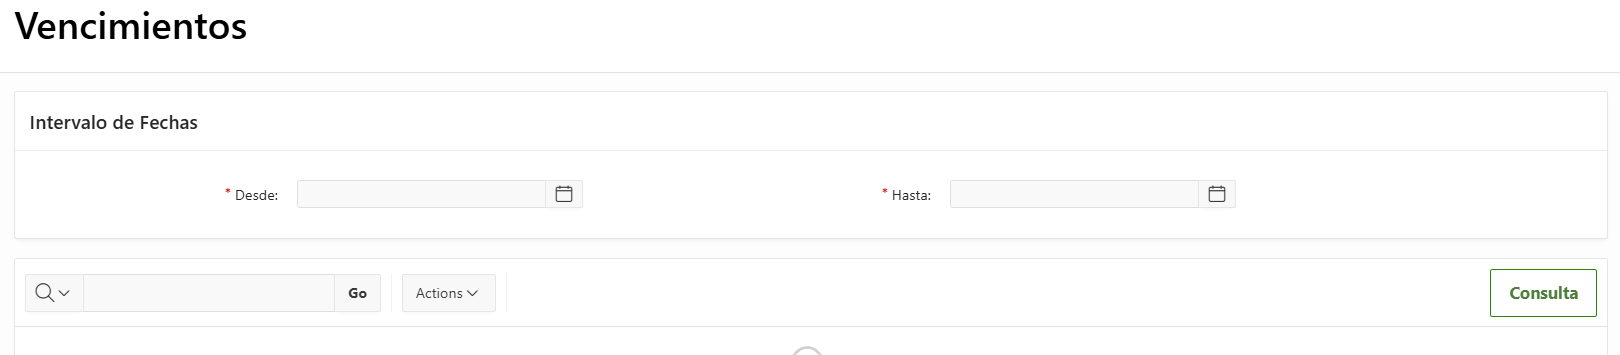
\includegraphics[width=5.90556in,height=1.36111in]{34.png}

Una vez pulsado el botón Buscar, se nos muestran las nóminas y el total de ese periodo. Este informe es usado para cotejar el importe pagado en un periodo a un contratado.

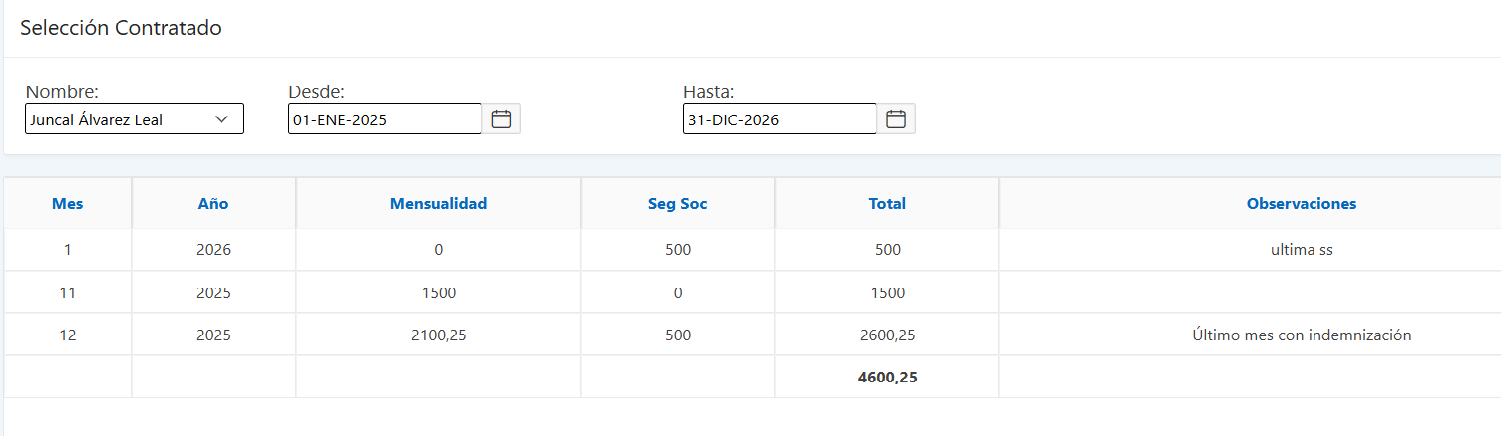
\includegraphics[scale=1]{35.png}

\section{Acerca de}\label{acerca-de}

Se muestran datos de la aplicación:\\

\includegraphics[scale=1]{36.png}

\subsection{Guía de uso}\label{guuxeda-de-uso}

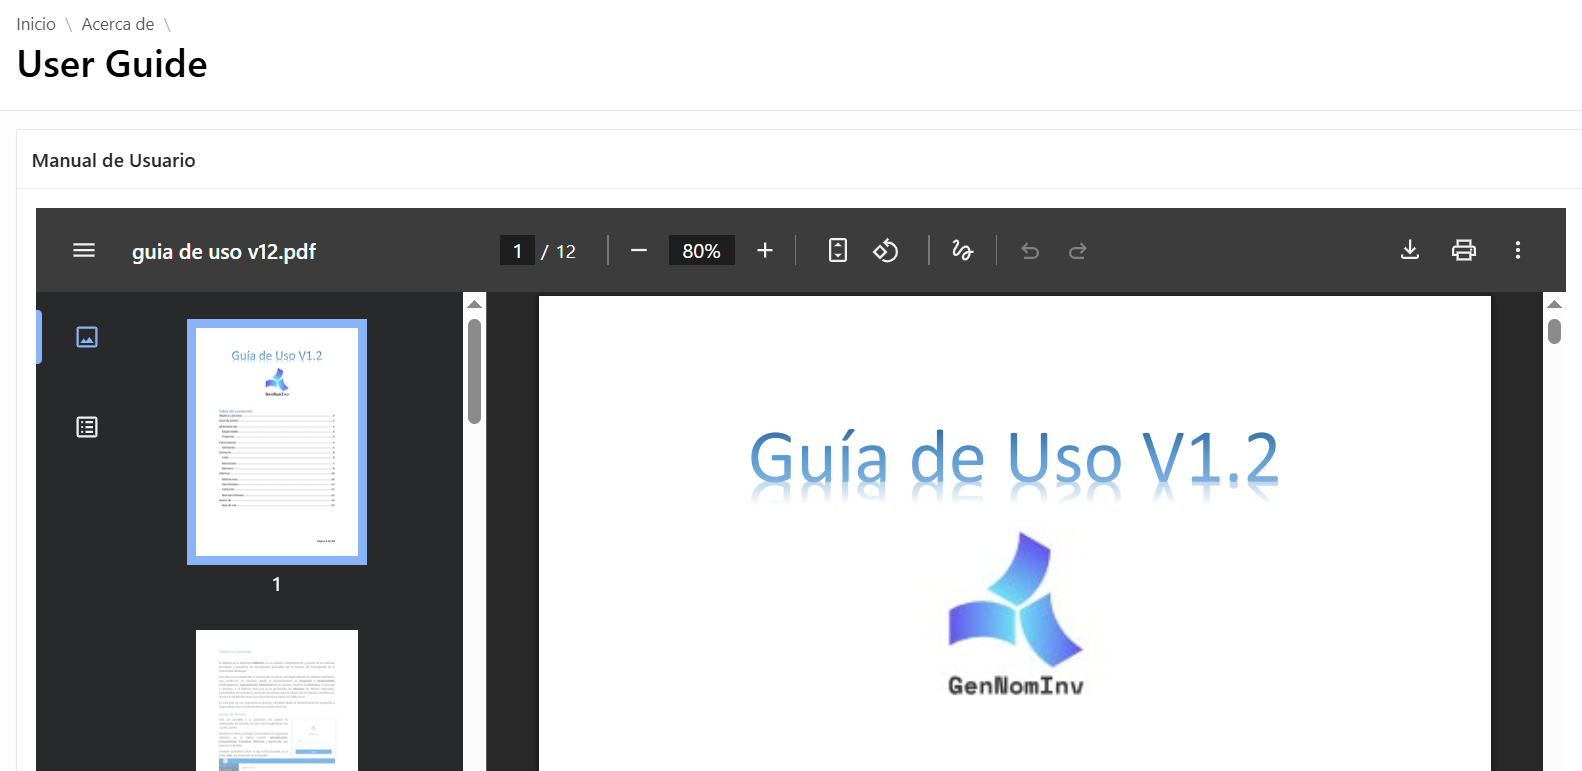
\includegraphics[width=5.1719in,height=2.14134in]{37.png}
